% !TeX encoding = UTF-8
% Lecture file created by newnote
% Class: Models of Theoretical Physics
% Professor: Azaele Sandro
% Date: 2025-10-14
\lecture{12}{Laplace method}{2025-10-14}
\pagelayout{margin}
% --- Start writing here ---

\section{Laplace method}
\begin{DispWithArrows}[displaystyle, format=c]
  I(\lambda) \simeq g\left(x_{0}\right) e^{\lambda f\left(x_{0}\right)} \sqrt{\frac{2 \pi}{\lambda\left|f^{\prime \prime}\left(x_{0}\right)\right|}}
\end{DispWithArrows}
interior max
$I(\lambda) \sim \lambda^{-1 / 2} e^{\lambda f\left(x_{0}\right)}$ endpoint (not
flat) $\quad I(\lambda) \sim \lambda^{-1} e^{\lambda f\left(x_{0}\right)}$

\subsection*{Lp-norm in real analysis}
The quantity
\begin{DispWithArrows}[displaystyle, format=c]
  \|g\|_{p}:=\left(\int_{a}^{b}|g(t)|^{p} d t\right)^{1 / p} \quad p>0
\end{DispWithArrows}
is called $p$-norm when the integral exists (in Lebesgue sense). We want to
study the behavior of $\|g\|_p$ as $p \rightarrow \infty$. We assume that $g$ has
a unique maximum in $t_{0}$ which is an interior point, and
$g \in C^{4}(a, b)$.
We first study
\begin{DispWithArrows}[displaystyle, format=c]
  I(p) \equiv \int_{a}^{b}|g(t)|^{p} d t \quad \|g\|_{p}=I(p)^{1 / p}
\end{DispWithArrows}
and
\begin{DispWithArrows}[displaystyle, format=c]
  I(p)=\int_{a}^{b} e^{p \ln |g(t)|} d t
\end{DispWithArrows}
When we applied the Laplace method we have always assumed that $f$ is
continuously differentiable. However, if $g$ vanishes somewhere in $[a, b]$
then $\ln|g| \rightarrow-\infty$. However, every neighborhood of points where
$g=0$ will yield a negligible contribution to the integral (i.e. to I for
$p \gg 1$).

Thus such discontinuities can be neglected. Now we use eq. (22) from the
previous lecture:
\begin{DispWithArrows}[displaystyle, format=c]
  \begin{aligned}
    I(p) & =e^{p \ln \left|g\left(t_{0}\right)\right|} \sqrt{\frac{2 \pi \left|g\left(t_{0}\right)\right|}{p\left|g^{\prime \prime}\left(t_{0}\right)\right|}}\left(1+O\left(\frac{1}{p}\right)\right) \\
    & =\left|g\left(t_{0}\right)\right|^{p} \sqrt{\frac{2 \pi \left|g\left(t_{0}\right)\right|}{p\left|g^{\prime \prime}\left(t_{0}\right)\right|}}\left(1+O\left(\frac{1}{p}\right)\right) \text { as } p \rightarrow \infty
  \end{aligned}
\end{DispWithArrows}
Obs: $\quad a>0 \quad a^{1 / p} p^{-\frac{1}{2 p}}=e^{\frac{\ln a}{p}} e^{-\frac{\ln p}{2 p}}$
\begin{DispWithArrows}[displaystyle, format=c]
  I(p)^{1 / p}=\left|g\left(t_{0}\right)\right|\left(\frac{2 \pi|g|}{p\left|g^{\prime \prime}\right|}\right)^{\frac{1}{2 p}}+...=\left|g\left(t_{0}\right)\right|\left(1-\frac{\ln p}{2 p}+O\left(\frac{1}{p}\right)\right)
\end{DispWithArrows}
hence
\begin{DispWithArrows}[displaystyle, format=c]
  \|g\|_{p}=\max _{t \in[a, b]}|g(t)|\left\{1-\frac{\ln p}{2 p}+\cdots\right\} \text { as } p \rightarrow \infty
\end{DispWithArrows}
which justifies the usual definition
\begin{DispWithArrows}[displaystyle, format=c]
  \|g\|_{\infty}=\max _{t \in[a, b]}|g(t)|
\end{DispWithArrows}
\subsection*{Example}
Consider the integral
\begin{DispWithArrows}[displaystyle, format=c]
  \int_{0}^{\frac{3 \pi}{2}} e^{-\lambda \sin t} f(t) d t \quad \text { as } \quad \lambda \rightarrow \infty
\end{DispWithArrows}
where $f$ is cont. and diff. in $\left[0, \frac{3 \pi}{2}\right]$.
\begin{figure}[H]
  \centering
  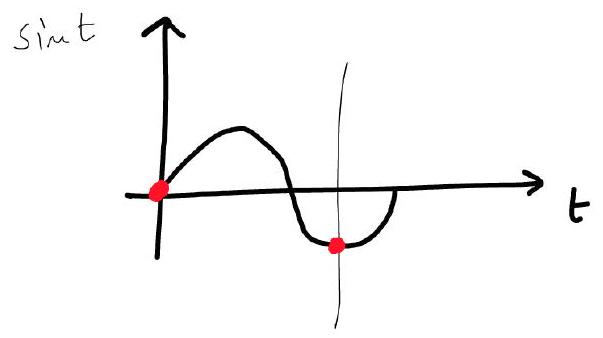
\includegraphics[width=0.5\textwidth]{graphics/2025_10_19_11b40f5928aca93f9d20g-3}
\end{figure}
We want to consider the contributions from the endpoint minima
$t=0, t=\frac{3 \pi}{2}$. For this we write
\begin{DispWithArrows}[displaystyle, format=c]
  I(\lambda)=\underbrace{\int_{0}^{\pi / 2} e^{-\lambda \sin t} f(t) d t}_{I_{1}}+\underbrace{\int_{\pi / 2}^{3 \pi / 2} e^{-\lambda \sin t} f(t) d t}_{I_{2}}
\end{DispWithArrows}
eqeq(24) left end point
\begin{DispWithArrows}[displaystyle, format=c]
  I_{1} \simeq f(0) \frac{e^{-\lambda \sin(0)}}{\lambda \cos (0)}=\frac{f(0)}{\lambda} \text { as } \lambda \rightarrow \infty
\end{DispWithArrows}
eqeq(23) flat endpoint
\begin{DispWithArrows}[displaystyle, format=c]
  I_{2} \simeq f\left(\frac{3 \pi}{2}\right) e^{\lambda} \sqrt{\frac{\pi}{2 \lambda\left|\sin \left(\frac{3 \pi}{2}\right)\right|}} = f\left(\frac{3 \pi}{2}\right) e^{\lambda} \sqrt{\frac{\pi}{2 \lambda}}
\end{DispWithArrows}
Hence the leading contribution comes from $I_{2}$ and
\begin{DispWithArrows}[displaystyle, format=c]
  I(\lambda) \simeq f\left(\frac{3 \pi}{2}\right) e^{\lambda} \sqrt{\frac{\pi}{2 \lambda}} \quad \text { as } \quad \lambda \rightarrow \infty
\end{DispWithArrows}
The min at $t=0$ is subleading and it should be taken into account only at
higher order.

Ex: Calculate the leading contribution to
\begin{DispWithArrows}[displaystyle, format=c]
  \int_{0}^{\pi} e^{-\lambda \sin t} f(t) d t \quad \text { as } \lambda \rightarrow \infty
\end{DispWithArrows}

\section{Review of Dynamical Systems}
In many applications (physics, biology, chemistry...) one has to study
nonlinear systems of (autonomous) ODEs:
\begin{DispWithArrows}[displaystyle, format=ll]
  \left\{\begin{aligned}
      \dot{\vec{x}}(t)&=\vec{f}(\vec{x}(t)) \\
      \vec{x}(0)&=\vec{x}_{0}
    \end{aligned}\right.
\end{DispWithArrows}
where $\vec{x}(t)=\left(x_{1}(t), \ldots, x_{N}(t)\right) \in U \subseteq \mathbb{R}^{N}, U$
is some open connected set of reals.
With any $\vec{x}$ we associate a vector $\vec{f}$, the set of these vectors is
called vector field. The domain $U$, where $\vec{f}$ is supposed to be
continuous and differentiable, is called the phase space.
The solutions $\vec{x}\left(t, x_{0}\right)$ of the system (1) describe smooth
curves as $t$ changes: they are called trajectories which are parametric curves
in the phase space.

\subsection*{Example:}
Let's consider ($N=1$)
\begin{DispWithArrows}[displaystyle, format=c]
  \dot{x}(t)=\sin [x(t)]
\end{DispWithArrows}
In this case the vector field is 1-dim. and coincides with the $x$-axis.
\begin{figure}[H]
  \centering
  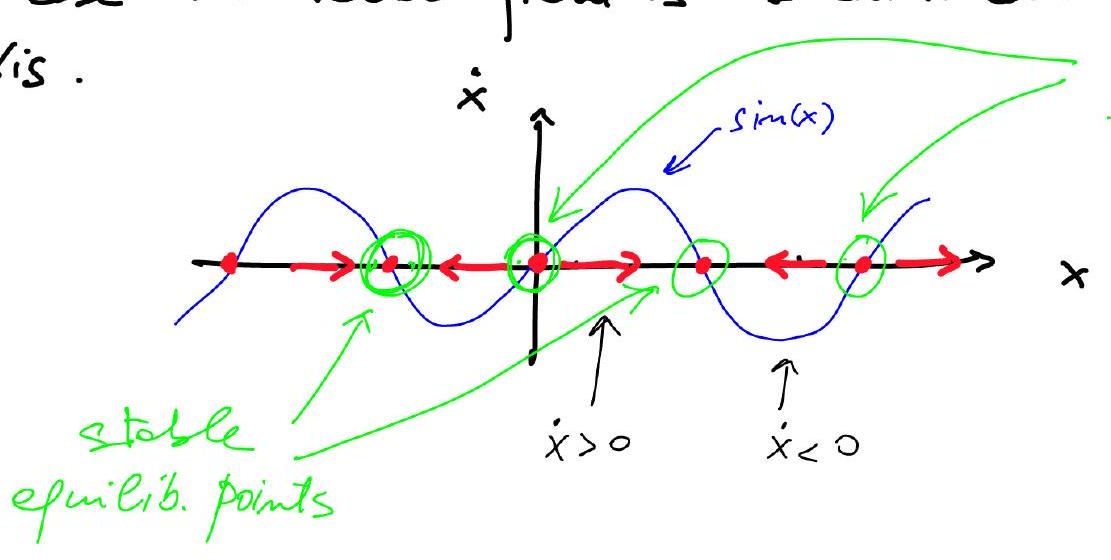
\includegraphics[width=0.5\textwidth]{graphics/2025_10_19_11b40f5928aca93f9d20g-4}
  \caption{equil. points}
\end{figure}
In the $N=2$ case
\begin{DispWithArrows}[displaystyle, format=ll]
  \left\{\begin{aligned}
      \dot{x}&=1 \\
      \dot{y}&=x^{2}+y^{2}
    \end{aligned}\right.
\end{DispWithArrows}
the vector field is 2 dim. and we have a map
\begin{DispWithArrows}[displaystyle, format=c]
  \vec{x}=(x, y) \longrightarrow \vec{f}(\vec{x})=\left(1, x^{2}+y^{2}\right)
\end{DispWithArrows}
\begin{figure}[H]
  \centering
  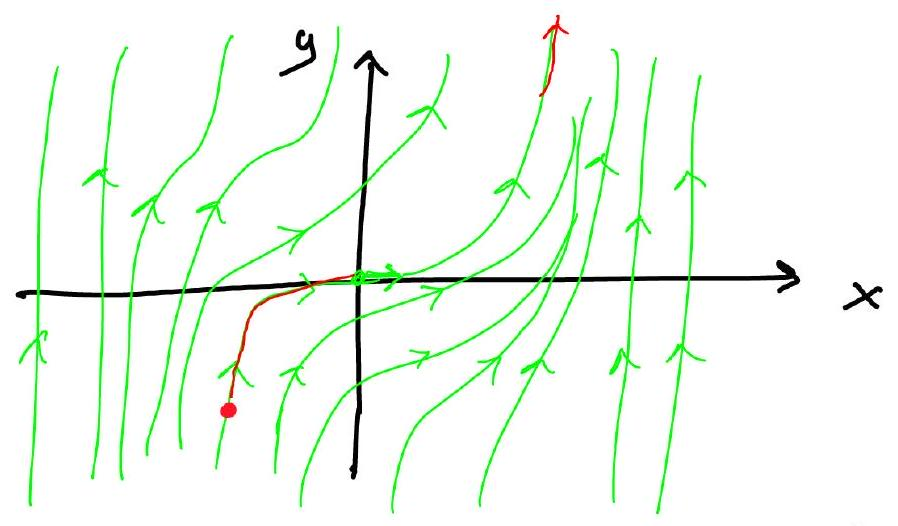
\includegraphics[width=0.5\textwidth]{graphics/2025_10_19_11b40f5928aca93f9d20g-5}
\end{figure}
In general the vector field $\vec{f}$ is tangent to a trajectory in every
point. In fact, let $\vec{x}(t)$ be a trajectory, then the eq. of a tangent
line to the trajectory at a point $\vec{x}_{a} \equiv \vec{x}\left(t_{a}\right)$
is
\begin{DispWithArrows}[displaystyle, format=c]
  \vec{Y}(u)=\vec{x}_{a}+\left(u-t_{a}\right) \dot{\vec{x}}\left(t_{a}\right)=\vec{x}_{a}+\left(u-t_{a}\right) \vec{f}\left(\vec{x}_{a}\right)
\end{DispWithArrows}
thus $\vec{f}$ is the directional vector of the straight line $\vec{Y}(u)$.
\begin{figure}[H]
  \centering
  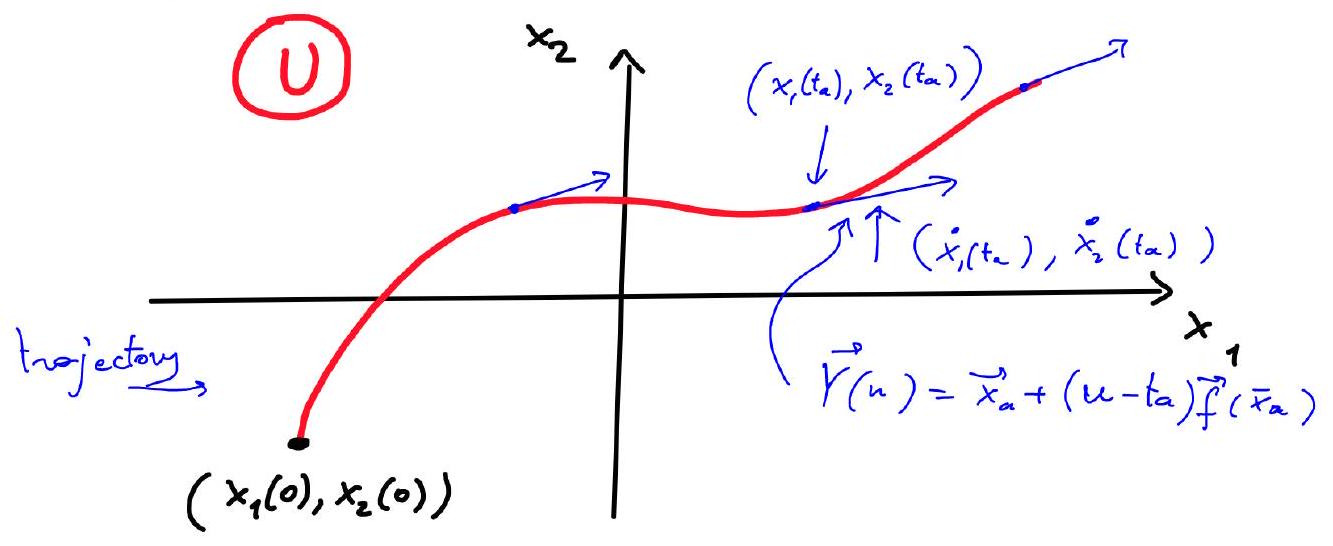
\includegraphics[width=0.5\textwidth]{graphics/2025_10_19_11b40f5928aca93f9d20g-5(1)}
\end{figure}
\begin{DispWithArrows}[displaystyle, format=ll]
  N=2 \ \left\{\begin{aligned}
      \dot{x}_{1}&=f_{1}\ \
      \dot{x}_{2}&=f_{2}
    \end{aligned}\right.
\end{DispWithArrows}
By flowing along the vector field, a point traces out the trajectory
$\vec{x}(t)$, a curve in the phase space $U$ or a sol. of (2).

A phase portrait is a set of trajectories with the indication of the directions
of the vector field.
As we cannot solve the system (1) in general, we would like to know at least
some properties.
Sometimes it is useful to study nullclines, defined as subspaces (or manifolds)
where $\dot{x}_{i}=0$ for a given i. In $N=2$ we may get simple curves
\begin{DispWithArrows}[displaystyle, format=c]
  \dot{x}_{1}=0 \Rightarrow f_{1}(x_1,x_2)=0 \text { possibly } x_{2}=g(x_1)
\end{DispWithArrows}
Two interesting examples
\begin{enumerate}
  \item Find a solution of $\dot{y}=y^{2}$ with i.c. $y(0)=1$.
\end{enumerate}
Can we then find $y(2)$?
From $\int \frac{d y}{y^{2}}=t-c, y=\frac{1}{c-t}, y(0)=1 \Rightarrow c=1$
\begin{DispWithArrows}[displaystyle, format=c]
  y(t)=\frac{1}{1-t} \quad \rightarrow y(2)=-1
\end{DispWithArrows}
As $\dot{y}(t) \geqslant 0, y$ is an increasing function of time but
$y(2)=-1$! Actually, the solution exists only in the interval $(0,1)$ as it
blows up at $t=1$.
Solutions may exist only within finite intervals of time or they may not exist
for some initial conditions or may not exist at all.
\begin{enumerate}
  \setcounter{enumi}{1}
  \item Find a solution of $\dot{y}=\sqrt{y}$ for which $y(0)=0$. Find $y(2)$. 
\end{enumerate}
\begin{DispWithArrows}[displaystyle, format=c]
  \int \frac{d y}{\sqrt{y}}=2 \sqrt{y}=t-c, \quad y=\frac{(t-c)^{2}}{4} \text { but } y(0)=0, y(t)=\frac{t^{2}}{4}
\end{DispWithArrows}
hence $y(2)=1$. But!

However $y(t)=0$ satisfies the eq. and the init. cond. Even worse:
\begin{DispWithArrows}[displaystyle, format=ll]
  y(t)=\left\{\begin{aligned}
      0 \quad 0 &\leq t \leq T & T \text { is arbitrary } \\
      \frac{(t-T)^{2}}{4} \quad &t>T & T>0 .
    \end{aligned}\right.
\end{DispWithArrows}
is a solution with the same initial condition! So there are infinitely many
solutions, so asking for $y(2)$ is meaningless.
Sol. to init. val problems may not be unique.

\subsection*{Picard's theorem}
If $\vec{f}$ is continuous and $\frac{\partial f_{i}}{\partial x_{j}}$ are also
continuous for all indexes $i,j$ in $U$, then for any $\vec{x}_{0} \in U$ the
initial value problem defined in (1) admits a solution on some interval
$t \in[-\delta, \delta], \delta>0$, and this solution is unique.

Obs: in this case trajectories do not intersect.

\subsection*{Fixed points}
The fixed points of eq. (1) are the simplest to study as time is not relevant.
Indeed, fixed points are the zeros of $\vec{f}$: namely, $\vec{x}^{*}$ is a
fixed point if
\begin{DispWithArrows}[displaystyle, format=c]
  \vec{f}\left(\vec{x}^{*}\right)=\overrightarrow{0}
\end{DispWithArrows}
Warning: even though an ODE has some fixed points, that does not imply that the
dynamics (the init. val. solut.) reach them!
